%%%%%%%%%%%%%%%%%%%%%%%%%%%%%%%%%%%%%%%%%%%%%%%%%%%%%%%%%%%%%%%%%%%%%%%%%%%%
% SU thesis coverpages generator
% Works for S5, A4 and A3 format
% 2017 by M Kocic
%%%%%%%%%%%%%%%%%%%%%%%%%%%%%%%%%%%%%%%%%%%%%%%%%%%%%%%%%%%%%%%%%%%%%%%%%%%%

\documentclass[12pt]{article}
\usepackage[margin=0cm,nohead]{geometry}
\usepackage[active,pdftex,tightpage,delayed]{preview}

\usepackage[T1]{fontenc}

\usepackage[nofligs]{verdana}
\renewcommand{\rmdefault}{lmr}

%\usepackage{times}
%\usepackage[none]{hyphenat}

% \usepackage{fontspec}
% \newfontfamily\mysigfont{Zapfino.ttf}

\usepackage{tikz,amsmath,amssymb,mathtools,mathrsfs,bm,color,cancel,xcolor}
\usepackage[colorlinks=true]{hyperref}
\usepackage{setspace}

\PreviewEnvironment{tikzpicture}
\setlength\PreviewBorder{0mm}

\usetikzlibrary{shapes,arrows}
\usetikzlibrary{calc}
\usetikzlibrary{positioning}
\usetikzlibrary{decorations.pathreplacing}
\usetikzlibrary{decorations.markings}
\usetikzlibrary{decorations.pathmorphing}

%%%%%%%%%%%%%%%%%%%%%%%%%%%%%%%%%%%%%%%%%%%%%%%%%%%%%%%%%%%%%%%%%%%%%%%%%%%%
% Parameters
%%%%%%%%%%%%%%%%%%%%%%%%%%%%%%%%%%%%%%%%%%%%%%%%%%%%%%%%%%%%%%%%%%%%%%%%%%%%

\newif\ifDebug          % \Debugtrue
\newif\ifHardcover      % \Hardcovertrue
\newif\ifPlastcover     % \Plastcovertrue
\newif\ifSoftcover      % \Softcovertrue
\newif\ifShowTemplate   % \ShowTemplatetrue
\newif\ifTightClip      % \TightCliptrue
\newif\ifClipFront      % \ClipFronttrue
\newif\ifClipBack       % \ClipBacktrue
\newif\ifShowAbstract     \ShowAbstracttrue

\def\PaperH{24.2}       % Paper height
\def\ExtraH{1}          % Extra height

\def\PaperW{16.5}       % Paper width
\def\ExtraW{1}          % Extra width

\def\SpineW{1}          % Spine width

\def\OffsetF{0}         % Text offset
\def\OffsetB{0}         % Text offset

\definecolor{suColor}{rgb}{0,0.184,0.373}

\definecolor{suSky}{rgb}{0.675,0.871,0.902}
\definecolor{suWater}{rgb}{0.608,0.698,0.808}
\definecolor{suWater2}{rgb}{0.557,0.722,0.863}

\newif\ifHScover
\ifHardcover\HScovertrue\fi
\ifSoftcover\HScovertrue\fi

\ifPlastcover\Hardcovertrue\fi

%%%%%%%%%%%%%%%%%%%%%%%%%%%%%%%%%%%%%%%%%%%%%%%%%%%%%%%%%%%%%%%%%%%%%%%%%%%%
% Hardcover fixup
%%%%%%%%%%%%%%%%%%%%%%%%%%%%%%%%%%%%%%%%%%%%%%%%%%%%%%%%%%%%%%%%%%%%%%%%%%%%

% Rules:
% ------
%   width  of cover = width  of text block - 1/8" = 3.2  mm
%   height of cover = height of text block + 1/4" = 6.35 mm
%   space between spine and cover = 1/4"..3/16" + thickness of the bookboard
%   spine width = text block width + 2 * thickness of the bookboard

% Calculations:
% -------------
%   text block width   =  167 mm
%   text block height  =  242 mm
%   board thickness    =  2 mm
%   cover width        =  170 mm
%   cover height       =  248 mm
%   space spine/cover  =  8 mm
%   spine width        =  9.5 + 2 * 2 mm = 13.5 mm

\ifHardcover
   \def\PaperW{17.2}    % Paper width
   \def\ExtraW{3.125}   % Extra width
   \def\ExtraH{2.75}    % Extra height
   \def\SpineW{1.35}    % Spine width for 2 mm Hardcover
   \def\OffsetF{0.7}    % Text offset on front
   \def\OffsetB{0.7}    % Text offset on back
   \def\BoardT{0.2}     % Bookboard thikness
   \def\BoardW{0.4}     % Width of board fold
   \definecolor{suColor}{rgb}{0,0.184,0.45}  % Konica SU printer
\fi

%%%%%%%%%%%%%%%%%%%%%%%%%%%%%%%%%%%%%%%%%%%%%%%%%%%%%%%%%%%%%%%%%%%%%%%%%%%%
% Softcover fixup
%%%%%%%%%%%%%%%%%%%%%%%%%%%%%%%%%%%%%%%%%%%%%%%%%%%%%%%%%%%%%%%%%%%%%%%%%%%%

\ifSoftcover
   \def\PaperW{16.6}   % Paper width
   \def\ExtraW{3}      % Extra width
   \def\ExtraH{2}      % Extra height
   \def\OffsetF{0.1}   % Text offset on front
   \def\OffsetB{0.1}   % Text offset on back
   \def\BoardT{0}      % Bookboard thikness
   \def\BoardW{0.1}    % Width of board fold
   \definecolor{suColor}{rgb}{0,0.184,0.45}  % Konica SU printer
\fi

%%%%%%%%%%%%%%%%%%%%%%%%%%%%%%%%%%%%%%%%%%%%%%%%%%%%%%%%%%%%%%%%%%%%%%%%%%%%

\begin{document}

\begin{tikzpicture}

  \node (A) at (-\PaperW - \SpineW, 0) {};
  \node (B) at (\PaperW, \PaperH) {};

  \ifHScover
     \clip ($(A)-(\ExtraW,34mm)$) 
         rectangle ($(B)+(\ExtraW,34mm)$);
  \else
     \clip ($(A)-(\ExtraW,\ExtraH)$) 
         rectangle ($(B)+(\ExtraW,\ExtraH)$);
  \fi
  
  \ifTightClip
     \clip (A) rectangle (B);
  \fi
  \ifClipFront
     \clip (0,0) rectangle (\PaperW,\PaperH);
  \fi
  \ifClipBack
     \clip (-\SpineW,0) rectangle (-\PaperW-\SpineW,\PaperH);
  \fi

  %%%%%%%%%%%%%%%%%%%%%%%%%%%%%%%%%%%%%%%%%%%%%%%%%%%%%%%%%%%%%%
  % FRONT COVER -- Artwork -- Bacground image
  %%%%%%%%%%%%%%%%%%%%%%%%%%%%%%%%%%%%%%%%%%%%%%%%%%%%%%%%%%%%%%
  
  % Include the artwork png (if you have it):
%  \node [anchor=south west,inner sep=0] at (0,1) 
%     {\includegraphics[height=134mm]{artwork.png}};

  % Default: show crowns
  
  \draw [color=white,fill=suWater2] (0,1) rectangle (20,14.4);
  \node [anchor=south,inner sep=0] at (6.6,8.4) 
      {
\includegraphics[width=70mm]{images/crown}};
  \node [anchor=south,inner sep=0] at (16.5,8.4) 
      {
\includegraphics[width=70mm]{images/crown}};
  \node [anchor=south,inner sep=0] at (11.55,1.6) 
      {
\includegraphics[width=78mm]{images/crown}};

  \ifHardcover
      \draw [color=white,line width=0,fill=white] (0,1)
         rectangle ++(0.025,\PaperH);
  \fi
  
  %%%%%%%%%%%%%%%%%%%%%%%%%%%%%%%%%%%%%%%%%%%%%%%%%%%%%%%%%%%%%%
  % FRONT COVER -- Frame
  %%%%%%%%%%%%%%%%%%%%%%%%%%%%%%%%%%%%%%%%%%%%%%%%%%%%%%%%%%%%%%
  
  \draw [suColor,opacity=0.2] (-\SpineW,0.85) -- (-\SpineW,1.3);
  \draw [suColor,opacity=0.2] (-\SpineW,20.95) -- (-\SpineW,21);
  
  \draw [color=suColor,fill=suColor] (-\PaperW-\ExtraW-\SpineW,21) 
      rectangle (\PaperW+\ExtraW,\PaperH+\ExtraH);
  \draw [color=suColor,fill=suColor] (-\PaperW-\ExtraW-\SpineW,-\ExtraH) 
      rectangle (\PaperW+\ExtraW,1.2);
  
  %%%%%%%%%%%%%%%%%%%%%%%%%%%%%%%%%%%%%%%%%%%%%%%%%%%%%%%%%%%%%%
  % FRONT COVER
  %%%%%%%%%%%%%%%%%%%%%%%%%%%%%%%%%%%%%%%%%%%%%%%%%%%%%%%%%%%%%%
  
  \node [anchor=south west, inner sep=0] 
    at (\OffsetF+13.05,21.25) {
	
\includegraphics[width=25mm]{images/SU-logo-white}};

  \node [anchor=south west, inner sep=0,text width=140mm] 
  at (\OffsetF+1.4,18.1) {%
     \fontsize{19.5}{1em}\selectfont%
     \textsf{\textbf{TITLE: the first line\\[3mm]
     the second line}}};

  \node [anchor=south west, align=left,text width=120mm,inner sep=0] 
  at (\OffsetF+1.4,17.2) {%
     \fontsize{14.5}{1em}\selectfont
     My Name};

  \node [white,anchor=south west, align=left,text width=130mm,inner sep=0] 
  at (\OffsetF+1.4,0.45) {%
    \fontsize{9}{0}\selectfont%
    Licentiate Thesis in Theoretical Physics at Stockholm University, 
    Sweden 2017};

  %%%%%%%%%%%%%%%%%%%%%%%%%%%%%%%%%%%%%%%%%%%%%%%%%%%%%%%%%%%%%%
  % BACK COVER
  %%%%%%%%%%%%%%%%%%%%%%%%%%%%%%%%%%%%%%%%%%%%%%%%%%%%%%%%%%%%%%
  
  \node [anchor=south west, inner sep=0] 
     at (-15.05-\SpineW-\OffsetB,1.85) {%
      
\includegraphics{images/fysikum}};

  \node [anchor=south west, inner sep=0] 
    at (-3.5-\SpineW-\OffsetB,1.9) {
	
\includegraphics[width=22mm]{images/SU-logo-blue}};

  \ifShowAbstract
    \node [anchor=north west,inner sep=0] 
      at (-15.05-\SpineW-\OffsetB,19.8) {%
      \begin{minipage}[t]{115mm}%
	    \rm\fontsize{10}{0}\selectfont%
	    \setlength{\baselineskip}{12.5pt}%\raggedright%
	    [Placeholder for abstract]\\[2mm]
	    \textsf{This is a coverpage template for Lic Thesis.}\\[1mm]
	    See: \texttt{cover/cover-page.tex}\\[2mm]
        \textbf{Usage}:\\[2mm]
        There are many flags to turn on/off:
        \begin{itemize}
        \item\texttt{\textbackslash{}Debugtrue} = Show debug frames
        \item\texttt{\textbackslash{}Hardcovertrue} = Show A3 for hardcover
        \item\texttt{\textbackslash{}Plastcovertrue} = Show A3 for plastic wrap
        \item\texttt{\textbackslash{}Softcovertrue} = Show A3 for softcover
        \item\texttt{\textbackslash{}ShowTemplatetrue} = Show the SU template
        \item\texttt{\textbackslash{}TightCliptrue} = Clip to S5 format strictly
        \item\texttt{\textbackslash{}ClipFronttrue} = Show only front cover
        \item\texttt{\textbackslash{}ClipBacktrue} = Show only back cover
        \item\texttt{\textbackslash{}ShowAbstracttrue} = Show abstract
        \end{itemize}
        You can insert your artwork pdf or png instead of crowns. \\[2mm]
        The template uses Verdana, but you can also insert PDFs 
        containing titles in Caecilia fonts
        (see 
        \url{http://www.su.se/medarbetare/visuellidentitet/identitetselement})
        \\[2mm]
		Regards, \\
		Mikica Kocic%
      \end{minipage}%
    };
  \fi

  %%%%%%%%%%%%%%%%%%%%%%%%%%%%%%%%%%%%%%%%%%%%%%%%%%%%%%%%%%%%%%
  % SPINE
  %%%%%%%%%%%%%%%%%%%%%%%%%%%%%%%%%%%%%%%%%%%%%%%%%%%%%%%%%%%%%%

  \node (S) at (0,19.7) {};

  \node [anchor=west,inner sep=0,rotate=-90] at ($(S)-(\SpineW/2,0)$) {%
    \fontsize{10}{1em}\selectfont%
    My Name};

  \node [anchor=west,inner sep=0,rotate=-90] at ($(S)-(\SpineW/2,3.65)$) {%
    \fontsize{10}{1em}\selectfont%\bfseries%
    The title visible on the spine};

  %%%%%%%%%%%%%%%%%%%%%%%%%%%%%%%%%%%%%%%%%%%%%%%%%%%%%%%%%%%%%%
  % Frame and template
  %%%%%%%%%%%%%%%%%%%%%%%%%%%%%%%%%%%%%%%%%%%%%%%%%%%%%%%%%%%%%%

  \ifShowTemplate
     \node [anchor=south,opacity=0.3,inner sep=0] at (-0.5,0) 
         {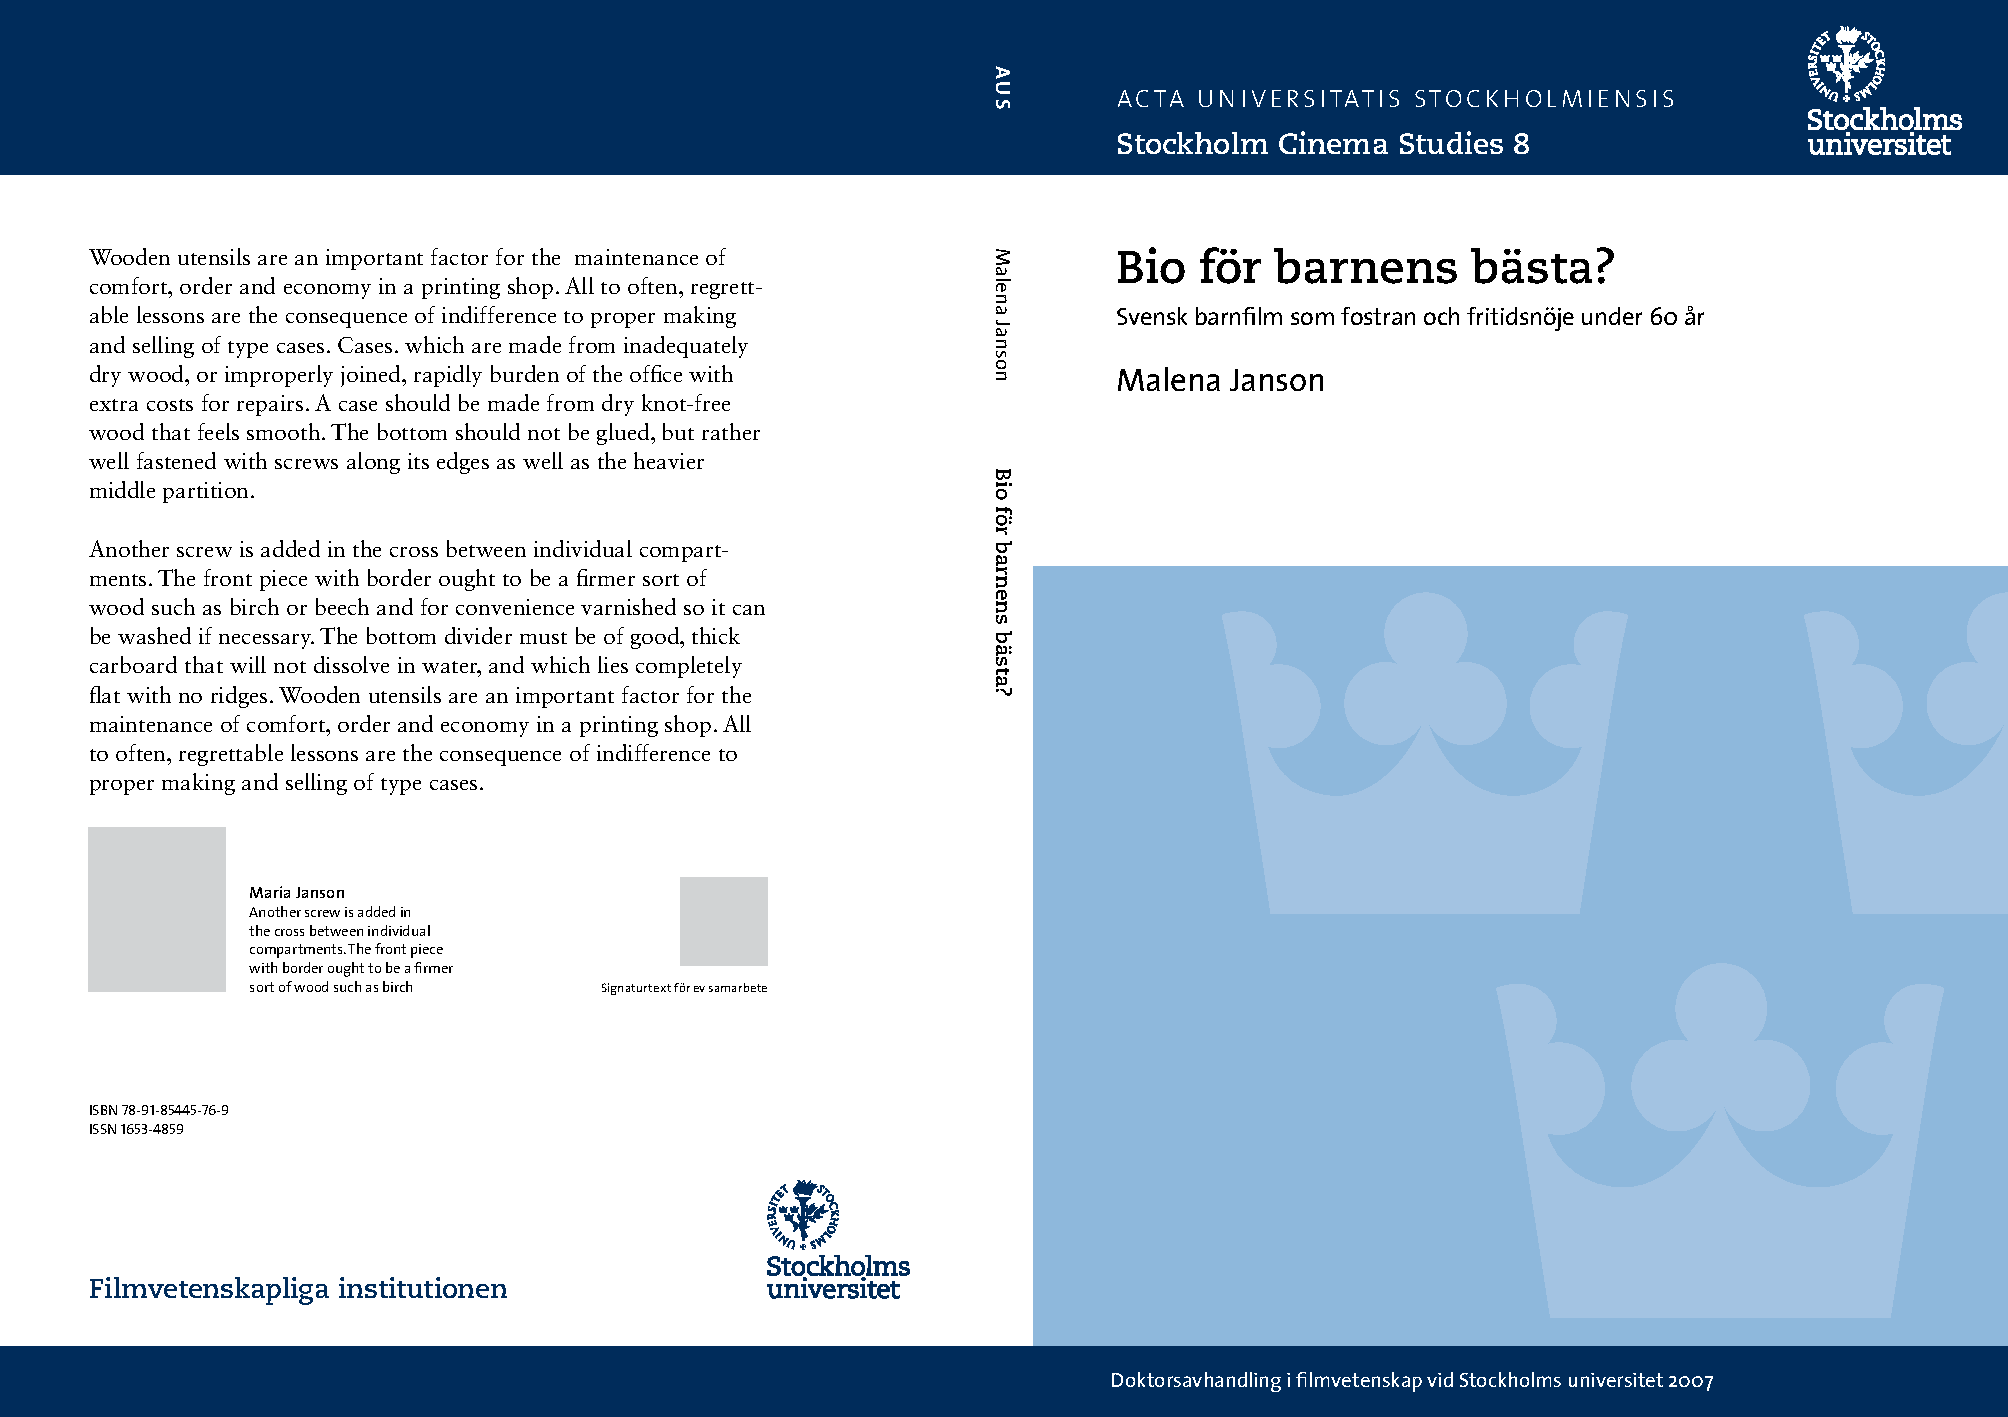
\includegraphics[width=340mm]{images/SU-avhandling-omslag-S5}};
  \fi

  \ifDebug
     \draw [green,dashed,thick] (0,0) rectangle (-\SpineW,\PaperH);
     \draw [red,dashed,thick] (A) rectangle (B);
     \draw [red,dashed,thick] ($(A)-(-0.01+\ExtraW,-0.01+\ExtraH)$) 
         rectangle ($(B)+(-0.01+\ExtraW,-0.01+\ExtraH)$);
  \fi

  \ifHScover
    \fill [white] (\PaperW+1,0) 
          rectangle ++(4,-4);
    \fill [white] (-\SpineW-\PaperW-1,0) 
          rectangle ++(-4,-4);
    \fill [white] (\PaperW+1,\PaperH) 
          rectangle ++(4,4);
    \fill [white] (-\SpineW-\PaperW-1,\PaperH) 
          rectangle ++(-4,4);

    \fill [white] (\BoardT,\PaperH+2*\ExtraH/3)
          rectangle ++(\BoardW+\BoardT,100mm);
    \fill [white] 
          (-\SpineW-\BoardW-2*\BoardT,\PaperH+2*\ExtraH/3)
          rectangle ++(\BoardW+\BoardT,100mm);
    \fill [white] (\BoardT,-2*\ExtraH/3)
          rectangle ++(\BoardW+\BoardT,-100mm);
    \fill [white] 
          (-\SpineW-\BoardW-2*\BoardT,-2*\ExtraH/3)
          rectangle ++(\BoardW+\BoardT,-100mm);

    \draw [red] (-30,-2.5) -- (30,-2.5);
    \draw [red] (-30,\PaperH+2.5) -- (30,\PaperH+2.5);

    \draw [red,line width=0,fill=white] (0,\PaperH+\ExtraH/2)
          rectangle ++(-\SpineW,100mm);
    \draw [red,line width=0,fill=white] (0,-\ExtraH/2)
          rectangle ++(-\SpineW,-100mm);

    \node [inner sep=3mm,rotate=-90] 
        at (-\SpineW/2,-\ExtraH+0.6) {%
        \pgfmathparse{10 * \SpineW}%
        \texttt{\pgfmathprintnumber{\pgfmathresult}}%
     };
        
    \ifDebug
      \draw [orange,thick,dashed] (\BoardT,0)
         -- ++(0,\PaperH);
      \draw [orange,thick,dashed] (\BoardW+2*\BoardT,0)
         -- ++(0,\PaperH);
      \draw [cyan,thick,dashed] (\BoardW+3*\BoardT,0)
         -- ++(0,\PaperH);
      \draw [orange,thick,dashed] (-\SpineW-\BoardT,0)
         -- ++(0,\PaperH);
      \draw [orange,thick,dashed] (-\SpineW-\BoardW-2*\BoardT,0)
         -- ++(0,\PaperH);
      \draw [cyan,thick,dashed] (-\SpineW-\BoardW-3*\BoardT,0)
         -- ++(0,\PaperH);
    \fi
  \fi

\end{tikzpicture}

%%%%%%%%%%%%%%%%%%%%%%%%%%%%%%%%%%%%%%%%%%%%%%%%%%%%%%%%%%%%%%

\end{document}